\documentclass[CJKutf8,dvipsnames,table]{beamer}
\usepackage{hyperref}
\hypersetup{
  pdftitle={Signals and Systems},
  pdfauthor={Hong MingJian},
  pdfsubject={Introduction},
  pdfpagemode={FullScreen},
  colorlinks={true},
  linkcolor={blue},
}

%% https://tex.stackexchange.com/questions/47576/combining-ifxetex-and-ifluatex-with-the-logical-or-operation
\usepackage{ifxetex,ifluatex}
\newif\ifxetexorluatex % a new conditional starts as false
\ifnum 0\ifxetex 1\fi\ifluatex 1\fi>0
   \xetexorluatextrue
\fi
\usepackage{ifplatform}
\ifxetexorluatex
	\usepackage[slantfont,boldfont]{xeCJK}
	\ifwindows
		\setCJKmainfont{SimSun} % Windows默认中文字体:中易宋体
	\fi
	\ifmacosx
		\setCJKmainfont{STSong} % MacOS默认中文字体:华文宋体
	\fi
	\iflinux
		\setCJKmainfont{Noto Serif CJK SC} % Linux默认中文字体:思源宋体(By Adobe & Google)
	\fi
\else
	\usepackage{CJKutf8}
\fi

\usepackage[export]{adjustbox}
\usepackage{mathptmx} %pdfTeX error: pdflatex (file fmex9.pfb): cannot open Type 1 font file for reading
                                                 %https://forum.ubuntu.com.cn/viewtopic.php?t=269943
\usepackage{mathtools}
\usepackage[mathscr]{urwchancal}

\usetheme{Madrid}%{Warsaw}
\usecolortheme{default}

%gets rid of bottom navigation bars
\setbeamertemplate{footline}[page number]{}
%gets rid of navigation symbols
\setbeamertemplate{navigation symbols}{}

\begin{document}
\ifxetexorluatex\else
\begin{CJK*}{UTF8}{song}
\fi

  \title{数字信号处理}
  \subtitle{第5讲:傅立叶变换}
  \author{洪明坚}
  \institute{重庆大学软件学院}
  \date{\today}

  \AtBeginSection[]
  {
    \begin{frame}
      \frametitle{Outline}
      \tableofcontents[currentsection]
    \end{frame}
  }

  \frame{\titlepage}
  \frame{\frametitle{目录}\tableofcontents}
  
  \section{连续时间傅立叶变换}
  
  %% PAGE
  \begin{frame}
    \frametitle{引入}
    \begin{itemize}
    \item 周期为$T$的方波串 \\
	\begin{tabular}{ll}
	\raisebox{-.5\height}

    \begin{math}
x(t) = 
\left\{
    \begin {aligned}
         & 1 \quad & |t| < T_1 \\
         & 0 \quad & T_1 < |t| < T/2                  
    \end{aligned}
\right.
	\end{math}

&
    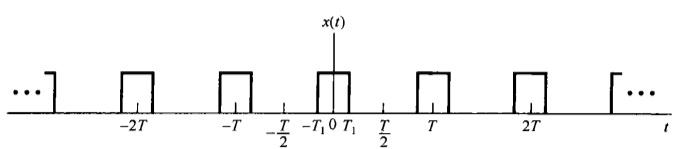
\includegraphics[valign=m,scale=.3]{ss-c-f4-1}    \\
    \end{tabular}  

  	\item 傅立叶级数的系数
   	\[ c_k = \frac{2sin(k\omega_0 T_1)}{k\omega_0 T}\] 
	可以写成
	\[
	Tc_k = \left. \frac{2sin(\omega T_1)}{\omega} \right\rvert_{\omega=k\omega_0}
	\]
	
    \end{itemize}      
  \end{frame}  

  %% PAGE
  \begin{frame}
    \frametitle{引入}
    \begin{itemize}
    \item $Tc_k$及其包络(envelop)曲线$\frac{2sin(\omega T_1)}{\omega}$的图像:(a)$T=4T_1$, (b)$T=8T_1$, (c)$T=16T_1$
		    \begin{center}
		   	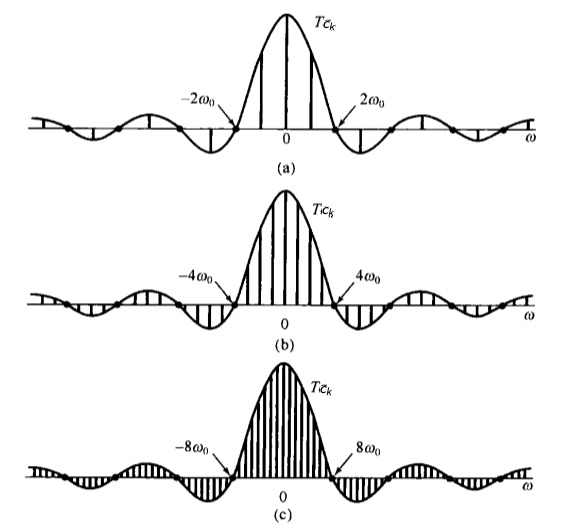
\includegraphics[scale=.27]{ss-c-f4-2}
    		\end{center}
	\item 固定$T_1$,随着$T$的增加,傅立叶系数是对包络曲线的越来越密集的采样。当$T \to \infty$时,一个非周期的方波函数的傅立叶系数趋近于该包络曲线。
    \end{itemize}

  \end{frame}    
   
  %% PAGE
  \begin{frame}
    \frametitle{定义}
    \begin{itemize}
    \item 对于任意函数$x(t)$,定义
    \begin{itemize}
    	\item 傅立叶变换
    	\[
			X(j\omega) = \int_{-\infty}^{\infty}x(t)e^{-j\omega t}dt    
    	\]
    	\item 傅立叶逆变换
    	\[
			x(t) = \frac{1}{2\pi}\int_{-\infty}^{\infty}X(j\omega)e^{j\omega t}d\omega    
    	\]    
    	\end{itemize}
    \end{itemize}

  \end{frame}     
   
  %% PAGE
  \begin{frame}
    \frametitle{傅立叶变换存在的充分条件}
    \begin{itemize}
    \item 能量条件
    \[
    	 \int_{-\infty}^{\infty}|x(t)|^2dt < \infty
    \]
    \item 波形条件
    \begin{itemize}
    	\item 绝对可积
    	\[
			\int_{-\infty}^{\infty}|x(t)|dt < \infty    
    	\]
    	\item 在任何有限区间内,只有有限个最大最小值
		\item 在任何有限区间内,只有有限个不连续点
   
    	\end{itemize}
    \end{itemize}

  \end{frame} 
     
  %% PAGE
  \begin{frame}
    \frametitle{例子}
    \begin{itemize}
    \item 指数函数
    \[
		x(t) = e^{at}u(t), a>0    
    \]
    \[
    	X(j\omega) = \int_{0}^{\infty}e^{-at}e^{-j\omega t}dt =\left. -\frac{1}{a+j\omega}e^{-(a+j\omega)t)} \right\rvert_{0}^{\infty} = \frac{1}{a+j\omega}
    \]
    
    	\begin{center}
      	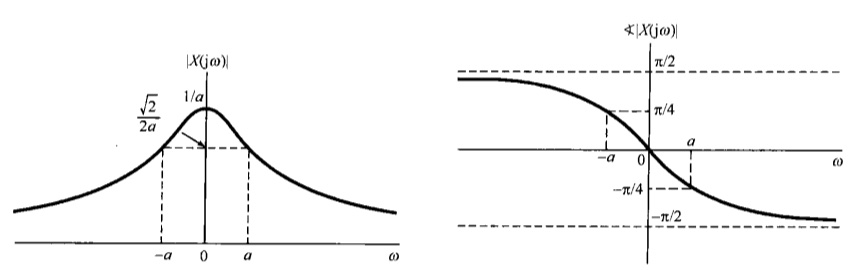
\includegraphics[scale=.37]{ss-c-f4-5}
    	\end{center}
    \end{itemize}

  \end{frame} 
     
  %% PAGE
  \begin{frame}
    \frametitle{例子}
    \begin{itemize}
    \item 高斯函数
    \[
		x(t) = e^{at^2}, a > 0    
    \]
    \[
    	X(j\omega) = \sqrt{\frac{\pi}{4}}e^{-\frac{\omega^2}{4a}}
    \]
    
    	\begin{center}
      	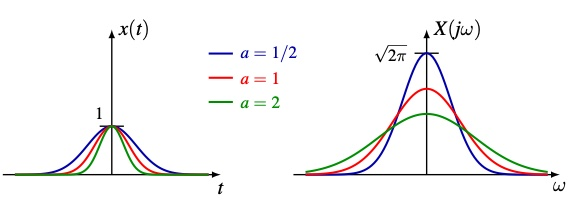
\includegraphics[scale=.5]{ftgaussian}
    	\end{center}
    \end{itemize}

  \end{frame} 
       
  %% PAGE
  \begin{frame}
    \frametitle{例子}
    \begin{itemize}
    \item 单位冲激函数$x(t) = \delta(t)$
    \[
    	X(j\omega) = \int_{-\infty}^{\infty}\delta(t)e^{-j\omega t}dt = 1
    \]
    逆变换
    \[
    	\delta(t) = \frac{1}{2\pi}\int_{-\infty}^{\infty}e^{j\omega t}d\omega
    \]
    \item DC信号$x(t)=1$    
    \[
    	X(j\omega) = \int_{-\infty}^{\infty}e^{-j\omega t}dt = \int_{-\infty}^{\infty}e^{j\omega t}dt = 2\pi\delta(\omega)
    \]
    逆变换
    \[
    	1 = \frac{1}{2\pi}\int_{-\infty}^{\infty}2\pi\delta(\omega)e^{j\omega t}d\omega
    \]
    \end{itemize}

  \end{frame} 

  %% PAGE
  \begin{frame}
    \frametitle{例子}
    \begin{itemize}    
    \item 复指数信号$x(t)=e^{j\omega_0 t}$
        \begin{align*}
 		X(j\omega) & = \int_{-\infty}^{\infty}e^{j\omega_0 t}e^{-j\omega t}dt \\
		& = \int_{-\infty}^{\infty}e^{j(\omega-\omega_0) t}dt    \\
		& = 2\pi\delta(\omega-\omega_0)
    	\end{align*} 
	逆变换
    \[
    	e^{j\omega_0 t} = \frac{1}{2\pi}\int_{-\infty}^{\infty}2\pi\delta(\omega-\omega_0)e^{j\omega t}d\omega
    \]

    \end{itemize}

  \end{frame}     
     
  %% PAGE
  \begin{frame}
    \frametitle{例子}
    \begin{itemize}
    \item 矩形脉冲函数
    \[
x(t) = 
\left\{
    \begin {aligned}
         & 1 \quad & |t| < T_1 \\
         & 0 \quad & otherwise                  
    \end{aligned}
\right.
	\]
	\[
		X(j\omega) = \int_{-T_1}^{T_1}e^{-j\omega t}dt = 2\frac{sin(\omega T_1)}{\omega}=2T_1sinc(\frac{\omega T_1}{\pi})
	\]
    
    	\begin{center}
      	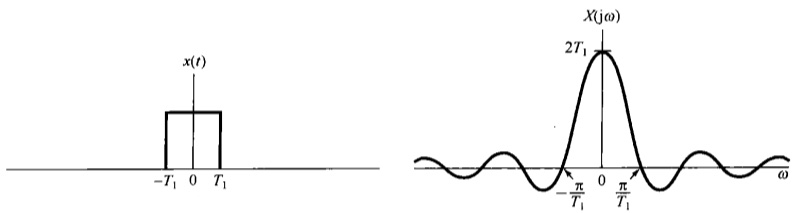
\includegraphics[scale=.37]{ss-c-f4-8}
    	\end{center}
	
		\begin{itemize}
		\item 其中
    	\[
    		sinc(\theta) = \frac{sin(\pi\theta)}{\pi\theta}
    	\]	
		\end{itemize}
    \end{itemize}

  \end{frame}      
     
  %% PAGE
  \begin{frame}
    \frametitle{例子}
    \begin{itemize}
    \item 反过来
    \[
X(j\omega) = 
\left\{
    \begin {aligned}
         & 1 \quad & |\omega| < W \\
         & 0 \quad & otherwise                  
    \end{aligned}
\right.
	\]
	\[
		x(t) = \frac{1}{2\pi}\int_{-W}^{W}e^{j\omega t}dt = \frac{sin(W t)}{\pi t} = \frac{W}{\pi}sinc(\frac{Wt}{\pi})
	\]
    
    	\begin{center}
      	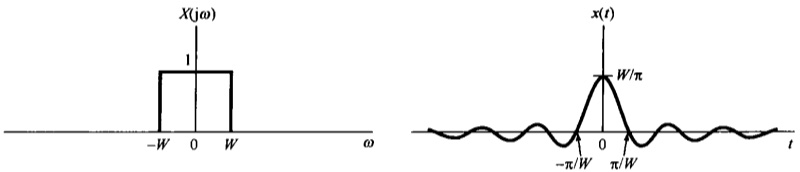
\includegraphics[scale=.37]{ss-c-f4-9}
    	\end{center}
	
		\begin{itemize}
		\item 其中
    	\[
    		sinc(\theta) = \frac{sin(\pi\theta)}{\pi\theta}
    	\]	
		\end{itemize}	
    \end{itemize}

  \end{frame} 
     
  %% PAGE
  \begin{frame}
    \frametitle{Questions}
    \begin{itemize}
    \item Any questions?
    \end{itemize}
    \begin{center}
      
\includegraphics[scale=.5]{question}
    \end{center}
  \end{frame} 
  
  \section{连续时间周期信号的傅立叶变换}
  
  %% PAGE
  \begin{frame}
    \frametitle{周期信号的傅立叶变换}
    \begin{itemize}
    \item 周期信号$x(t)$有傅立叶级数表示
    \[ 
    	x(t)=\sum_{k=-\infty}^{\infty}c_k e^{jk\omega_0 t} 
    \]
    \item 它的傅立叶变换
    	\begin{align*}
 		X(j\omega) & = \int_{-\infty}^{\infty}x(t)e^{-j\omega t}dt    \\
		& = \int_{-\infty}^{\infty}\sum_{k=-\infty}^{\infty}c_k e^{jk\omega_0 t}e^{-j\omega t}dt    \\
		& = \sum_{k=-\infty}^{\infty}c_k \int_{-\infty}^{\infty}e^{jk\omega_0 t}e^{-j\omega t}dt  \\
		& = \sum_{k=-\infty}^{\infty}2\pi c_k \delta(\omega-k\omega_0)
    	\end{align*}    
    \end{itemize}
  \end{frame}
  
  %% PAGE
  \begin{frame}
    \frametitle{例子:sin和cos}
    \begin{center}
      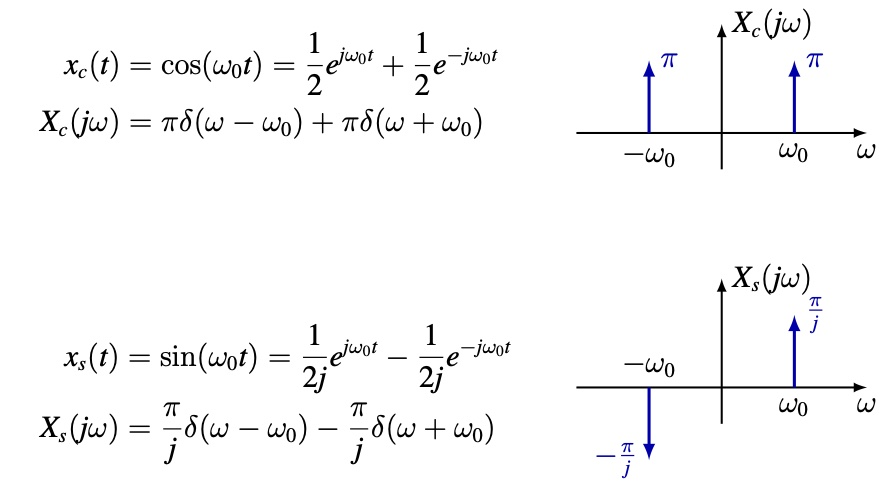
\includegraphics[scale=.4]{ftsincos}
    \end{center}    
  \end{frame}

  %% PAGE
  \begin{frame}
    \frametitle{例子:周期方波}
    \begin{center}
      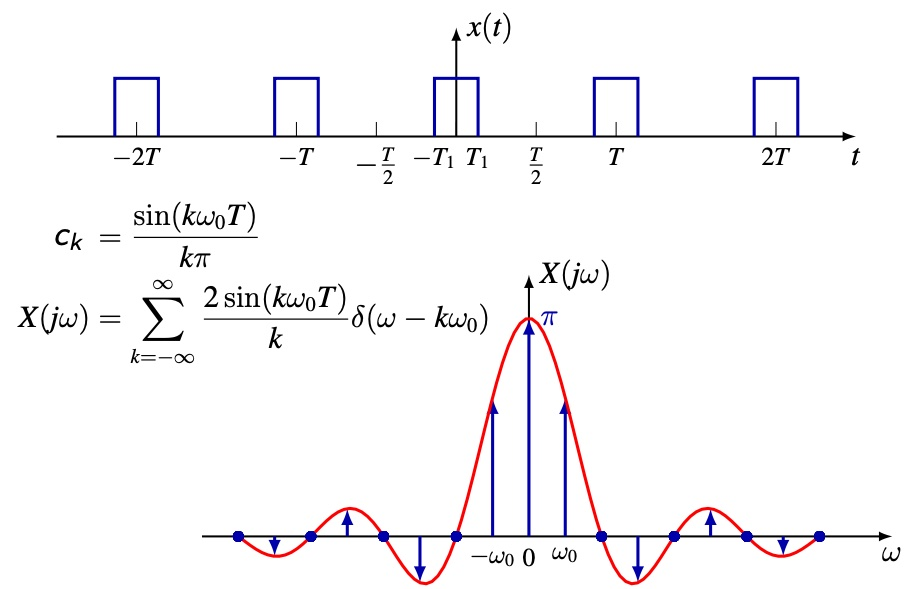
\includegraphics[scale=.35]{ftpsquare}
    \end{center}    
  \end{frame}    
    
  %% PAGE
  \begin{frame}
    \frametitle{例子:周期单位冲激串}
    \begin{center}
      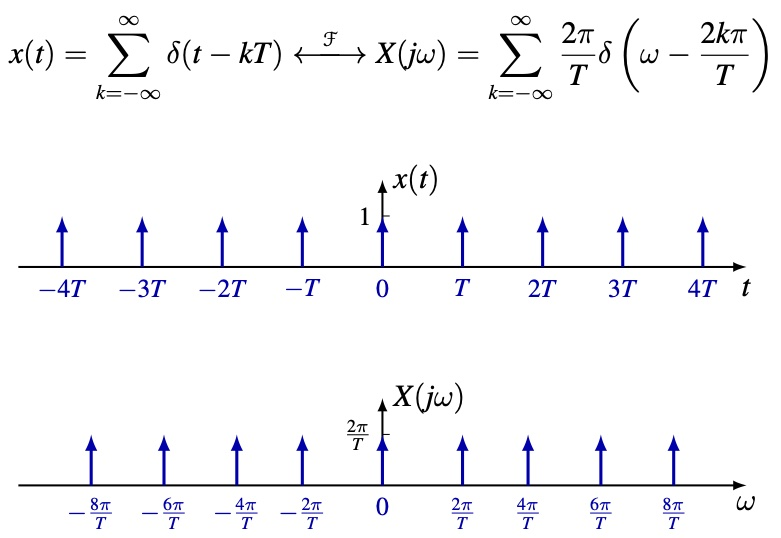
\includegraphics[scale=.35]{ftpimpulse}
    \end{center}    
  \end{frame}    
    
  %% PAGE
  \begin{frame}
    \frametitle{基本傅立叶变换对}
    \begin{center}
      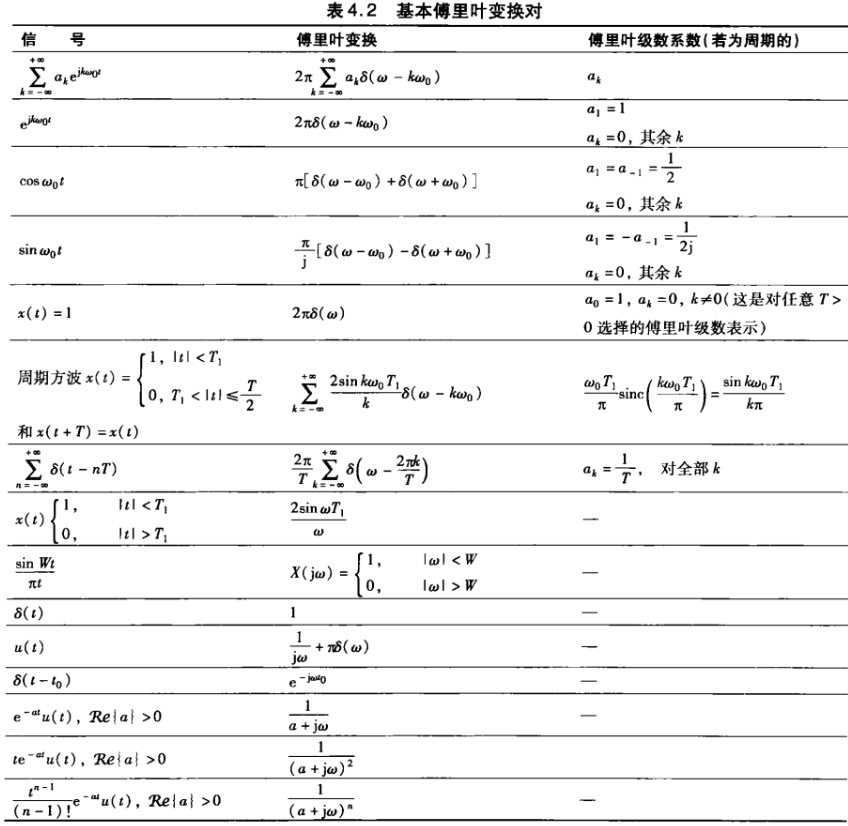
\includegraphics[scale=.29]{ss-c-t4-2}
    \end{center}
  \end{frame} 
    
  %% PAGE
  \begin{frame}
    \frametitle{Questions}
    \begin{itemize}
    \item Any questions?
    \end{itemize}
    \begin{center}
      
\includegraphics[scale=.5]{question}
    \end{center}
  \end{frame}   

	\section{连续时间傅立叶变换的性质}

  %% PAGE
  \begin{frame}
    \frametitle{性质}
    \begin{itemize}
    \item 线性:若$x(t) \xleftrightarrow{\mathscr{F}} X(j\omega)$, $y(t)\xleftrightarrow{\mathscr{F}}Y(j\omega)$,则
    \[
    ax(t)+by(t) \xleftrightarrow{\mathscr{F}} aX(j\omega)+bY(j\omega)
    \]
    \item 时移:$x(t-t_0) \xleftrightarrow{\mathscr{F}} e^{-j\omega t_0}X(j\omega)$
%    \item 共轭:$x^{*}(t) \xleftrightarrow{\mathscr{F}} X^{*}(-j\omega)$
    \item 微分:$\frac{dx(t)}{dt} \xleftrightarrow{\mathscr{F}} j\omega X(j\omega)$
%    \item 积分:$\int_{-\infty}^{t}x(\tau)d\tau \xleftrightarrow{\mathscr{F}} \frac{1}{j\omega} X(j\omega)+\pi X(0)\delta(\omega)$
%    \item 尺度变换:$x(at) \xleftrightarrow{\mathscr{F}} \frac{1}{|a|}X(\frac{j\omega}{a})$
	\end{itemize}
  \end{frame}    

  %% PAGE
  \begin{frame}
    \frametitle{性质}
    \begin{itemize}
    \item 对偶(Duality)
    	\begin{itemize}
		\item
\begin{align*}
    \delta(t) & \xleftrightarrow{\mathscr{F}} 1  \\        
        1 & \xleftrightarrow{\mathscr{F}} 2\pi\delta(\omega) 
\end{align*}    
		\item
\begin{align*}
\delta(t-t_0) & \xleftrightarrow{\mathscr{F}} e^{-j\omega t_0} \\
e^{j\omega_0 t} & \xleftrightarrow{\mathscr{F}} 2\pi\delta(\omega-\omega_0) 
\end{align*}   

		\item    
    		\begin{center}
      		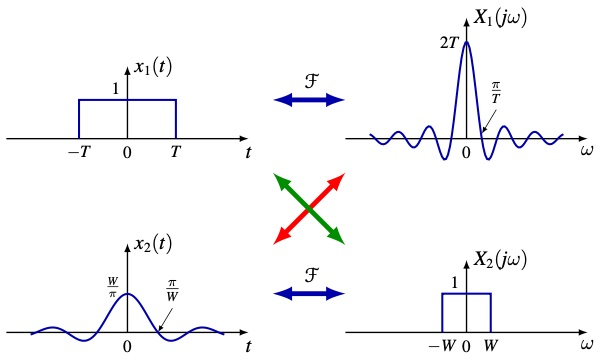
\includegraphics[scale=.3]{ftduality}
    		\end{center}
		\end{itemize}      
    \end{itemize}

  \end{frame}    

	
  %% PAGE
  \begin{frame}
    \frametitle{性质}
    \begin{itemize}
%    \item 帕斯瓦尔定理
%    \[
%    \int_{-\infty}^{\infty}|x(t)|^2dt=\frac{1}{2\pi}\int_{-\infty}^{\infty}|X(j\omega)|^2d\omega
%    \]
    \item 卷积
    \[
    	x_1(t) \ast x_2(t) \xleftrightarrow{\mathscr{F}} X_1(j\omega)X_2(j\omega)
    \]
    	\begin{itemize}
		\item 因为LTI系统的频率响应$H(j\omega)$是单位脉冲响应$h(t)$的傅立叶变换
		\[
			H(j\omega)=\mathscr{F}(h(t))=\int_{\mathbb{R}}h(t)e^{-j\omega t}dt
		\]
		所以
		\[
			x(t) \ast h(t) \xleftrightarrow{\mathscr{F}} X(j\omega)H(j\omega)
		\]
    	\end{itemize}

    \item 相乘
    \[
    	x_1(t)x_2(t) \xleftrightarrow{\mathscr{F}} \frac{1}{2\pi} \int_{-\infty}^{\infty}X_1(j\theta)X_2(j(\omega-\theta))d\theta = X_1(j\omega) \ast X_2(j\omega)
    \]    	
    \end{itemize}
  \end{frame}   
  	
  %% PAGE
  \begin{frame}
    \frametitle{例子}
    \begin{itemize}
    \item 理想低通滤波器 \\
	\begin{tabular}{ll}
	\raisebox{-.5\height}

    \begin{math}
H(j\omega) = 
\left\{
    \begin {aligned}
         & 1 \quad & |\omega| < \omega_c \\
         & 0 \quad & otherwise                  
    \end{aligned}
\right.
	\end{math}

&
    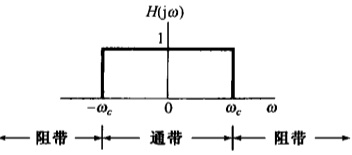
\includegraphics[valign=m,scale=.35]{ss-c-f4-20}    \\
    \end{tabular}      
    
    的单位冲激响应
    \[
    h(t)=\mathscr{F}^{-1}(H(j\omega))=\frac{sin(\omega_c t)}{\pi t}
    \]
    \begin{center}
      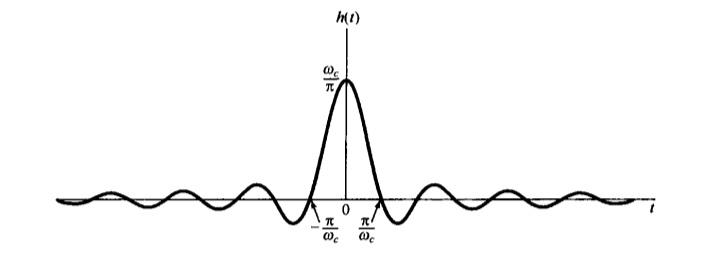
\includegraphics[scale=.4]{ss-c-f4-21}
    \end{center}
    因为$t<0$时$h(t)\neq 0$,所以该滤波器不是因果的
    
    \end{itemize}
  \end{frame}   

  %% PAGE
  \begin{frame}
    \frametitle{性质}
    \begin{itemize}
    \item 定义
    \[
    	p(t) = \frac{|x(t)|^2}{\int_R |x(\tau)|^2d\tau}, P(\omega) = \frac{|X(j\omega)|^2}{\int_R |X(j\theta)|^2d\theta}
    \]
    分别为时域和频域的归一化能量密度函数。
    \item 则$x(t)$和$X(j\omega)$的均值和标准差
    \begin{align*}
    	t_0 & = \int_R tp(t)dt, \Delta t = \sqrt{\int_R (t-t_0)^2 p(t)dt} \\
		\omega_0 & = \int_R \omega P(\omega)d\omega, \Delta \omega = \sqrt{\int_R (\omega-\omega_0)^2 P(\omega)d\omega}
    \end{align*}
	\begin{block}{测不准原理(Uncertainty principle)}
		$\Delta t \Delta \omega \geq \frac{1}{2}$,即信号不可能在时域和频域同时被准确定位。时域越短,频域越长;频域越短,时域越长。
	\end{block}	
    \end{itemize}
  \end{frame}   

  %% PAGE
  \begin{frame}
    \frametitle{性质汇总}
    \begin{center}
      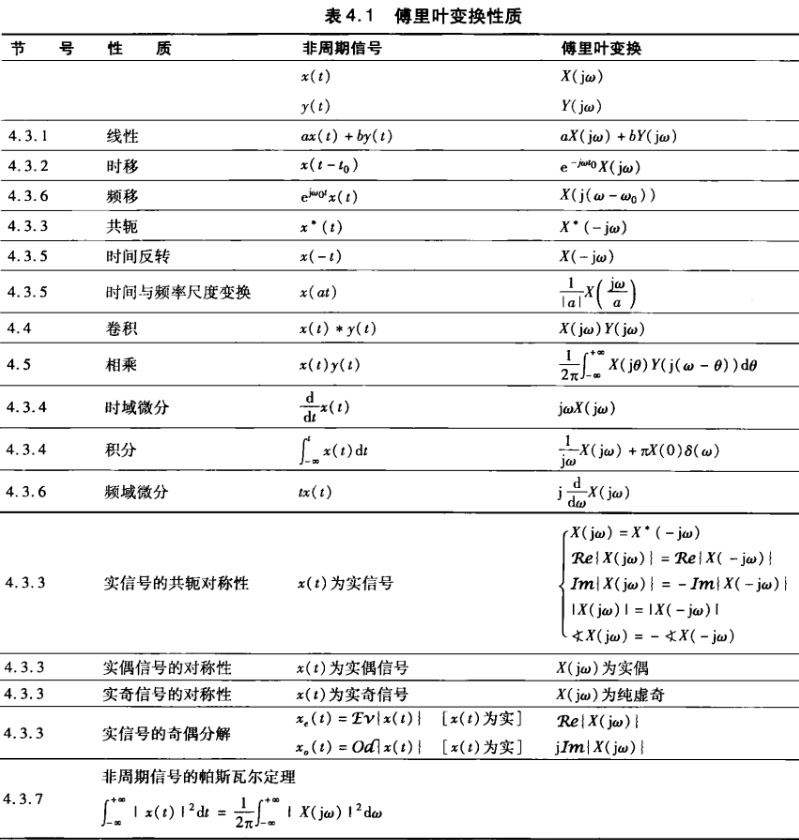
\includegraphics[scale=.28]{ss-c-t4-1}
    \end{center}
  \end{frame}  

  %% PAGE
  \begin{frame}
    \frametitle{Questions}
    \begin{itemize}
    \item Any questions?
    \end{itemize}
    \begin{center}
      
\includegraphics[scale=.5]{question}
    \end{center}
  \end{frame}  
  
  \section{离散时间傅立叶变换}

  %% PAGE
  \begin{frame}
    \frametitle{定义}
    \begin{itemize}
    \item 对于任意序列$x[n]$,定义
    \begin{itemize}
    	\item 傅立叶变换
    	\[
			X(e^{j\omega}) = \sum_{n=-\infty}^{\infty}x[n]e^{-j\omega n}    
    	\]
			\begin{itemize}
			\item 注意:$X(e^{j\omega})$以$2\pi$为周期
			\end{itemize}	
    	\item 傅立叶逆变换
    	\[
			x[n] = \frac{1}{2\pi}\int_{2\pi}X(e^{j\omega})e^{j\omega n}d\omega    
    	\]
    	\end{itemize}
    \end{itemize}

  \end{frame}   
       
  %% PAGE
  \begin{frame}
    \frametitle{例子}
    \begin{itemize}
    \item 矩形脉冲序列 \\
	\begin{tabular}{ll}
	\raisebox{-.5\height}

    \begin{math}
x[n] = 
\left\{
    \begin {aligned}
         & 1 \quad & |n| < N_1 \\
         & 0 \quad & otherwise                  
    \end{aligned}
\right.
	\end{math}

&
    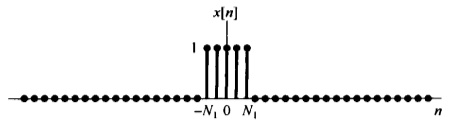
\includegraphics[valign=m,scale=.4]{ss-c-f5-6a}    \\
    \end{tabular} 
    
    \item
    \[
    X(e^{j\omega}) = \sum_{n=-N_1}^{N_1}e^{-j\omega n} = \frac{sin(\omega (N_1 + \frac{1}{2}))}{sin(\omega /2)}
    \]
    	\begin{center}
    	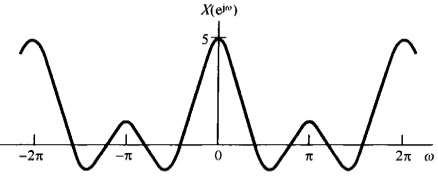
\includegraphics[scale=.5]{ss-c-f5-6b}
    	\end{center}    
		\begin{itemize}
		\item 注意:低频在$2k\pi$周围,而高频在$(2k+1)\pi$周围
		\end{itemize}
    \end{itemize}

  \end{frame}  
  
  %% PAGE
  \begin{frame}
    \frametitle{傅立叶变换存在的充分条件}
    \begin{itemize}
    \item 对于正变换,如果
    \[
    	 \sum_{n=-\infty}^{\infty}|x[n]| < \infty
    \]
    则$X(e^{j\omega})$存在
    	\begin{itemize}
		\item 因为LTI系统的频率响应$H(e^{j\omega})$是单位脉冲响应$h[n]$的傅立叶变换
		\[
			H(e^{j\omega})=\mathscr{F}(h[n])=\sum_n h[n]e^{-j\omega n}
		\]   
		\item 所以,如果一个LTI系统是稳定的,即
		\[
			\sum_n|h[n]| < \infty
		\]
		它的频率响应总是存在。		
		\end{itemize}
    \item 逆变换只涉及有限积分区间,一般不存在收敛性问题。
    
 
    \end{itemize}

  \end{frame} 
        
  %% PAGE
  \begin{frame}
    \frametitle{例子}
    \begin{itemize}
    \item 单位脉冲序列$x[n]=\delta[n]$的傅立叶变换$X(e^{j\omega})=1$
	\item 
	\[
	\hat{x}[n] = \frac{1}{2\pi}\int_{-W}^{W} e^{j\omega n}d\omega = \frac{sin(Wn)}{\pi n}
	\]    
    	\begin{center}
    	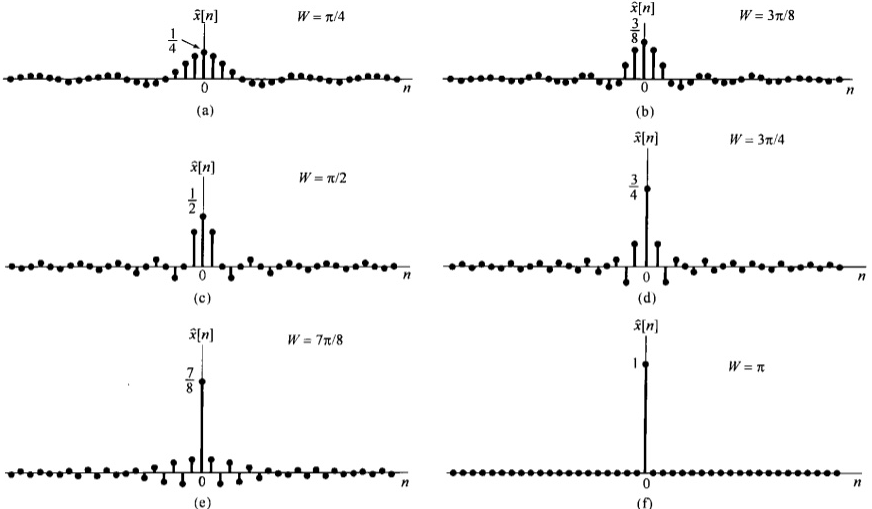
\includegraphics[scale=.3]{ss-c-f5-7}
    	\end{center}   
		\begin{itemize}
		\item 没有Gibbs现象!
		\end{itemize}
    \end{itemize}

  \end{frame}    
        
  %% PAGE
  \begin{frame}
    \frametitle{Questions}
    \begin{itemize}
    \item Any questions?
    \end{itemize}
    \begin{center}
      
\includegraphics[scale=.5]{question}
    \end{center}
  \end{frame}     
  
  \section{离散时间周期信号的傅立叶变换}

  %% PAGE
  \begin{frame}
    \frametitle{复指数信号}
    \begin{itemize}
    \item 周期为$N$的复指数信号
    \[
    	x[n]=e^{j\omega_0 n}, \omega_0=\frac{2\pi}{N}
    \]
    它的傅立叶变换
    \[
    	X(e^{j\omega})=\sum_{n=-\infty}^{\infty}e^{j\omega_0 n}e^{-j\omega n}=\sum_{l=-\infty}^{\infty}2\pi \delta(\omega - \omega_0 - 2\pi l)
    \]
    	\begin{center}
    	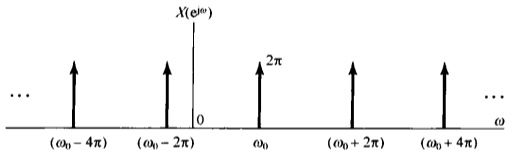
\includegraphics[scale=.4]{ss-c-f5-8}
    	\end{center}  
%	\item 注意
%		\begin{itemize}
%		\item 该信号不满足收敛的充分条件
%		\item 暂时只能通过傅立叶逆变换来验证正确性
%		\end{itemize}

    \end{itemize}
  \end{frame}     
  
  %% PAGE
  \begin{frame}
    \frametitle{一般的周期信号}
    \begin{itemize}
    \item 周期为$N$的$x[n]$可以做傅立叶级数展开
    \[
    	x[n] = \sum_{k=<N>} c_k e^{jk\omega_0 n}
    \]
    它的傅立叶变换
    \[
    	X(e^{j\omega})=\sum_{k=-\infty}^{\infty}2\pi c_k \delta(\omega - k\omega_0)
    \]
    \end{itemize}

  \end{frame}   
  
  %% PAGE
  \begin{frame}
    \frametitle{例子}
    \begin{itemize}
    \item 正弦信号
    \[
    	x[n]=cos(\omega_0 n)=\frac{1}{2}e^{jk\omega_0 n}+\frac{1}{2}e^{-jk\omega_0 n}
	\]
	\item 的傅立叶变换
        \begin{align*}
 		X(e^{j\omega}) & = \sum_{l=-\infty}^{\infty}\pi \delta(\omega - \omega_0 - 2\pi l)+\sum_{l=-\infty}^{\infty}\pi \delta(\omega + \omega_0 - 2\pi l) \\
		& = \pi \delta(\omega - \omega_0)+\pi \delta(\omega + \omega_0), -\pi \leq \omega < \pi   
    	\end{align*} 	
	
    	\begin{center}
    	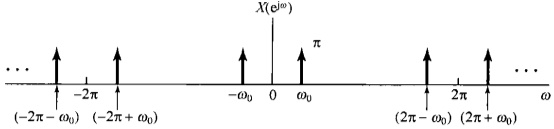
\includegraphics[scale=.5]{ss-c-f5-10}
    	\end{center}
    \end{itemize}

  \end{frame}    
  
  %% PAGE
  \begin{frame}
    \frametitle{例子}
    \begin{itemize}
    \item 周期单位冲激串
    \[
	    x[n]=\sum_{k=-\infty}^{\infty}\delta[n-kN]
    \]
    \item 的傅立叶级数系数
    \[
    	c_k=\frac{1}{N}\sum_{n=<N>}x[n]e^{-jk\omega_0 n}=\frac{1}{N}
    \]
	\item 因此
        \[
 			X(e^{j\omega}) = \frac{2\pi}{N}\sum_{k=-\infty}^{\infty}\delta(\omega - k\frac{2\pi}{N})   
    	\]	
	
    	\begin{center}
    	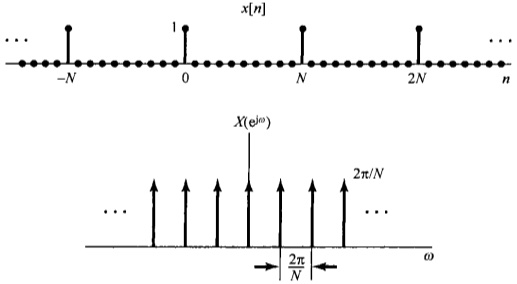
\includegraphics[scale=.35]{ss-c-f5-11}
    	\end{center}
    \end{itemize}

  \end{frame}    
    
  %% PAGE
  \begin{frame}
    \frametitle{基本傅立叶变换对}
    \begin{center}
      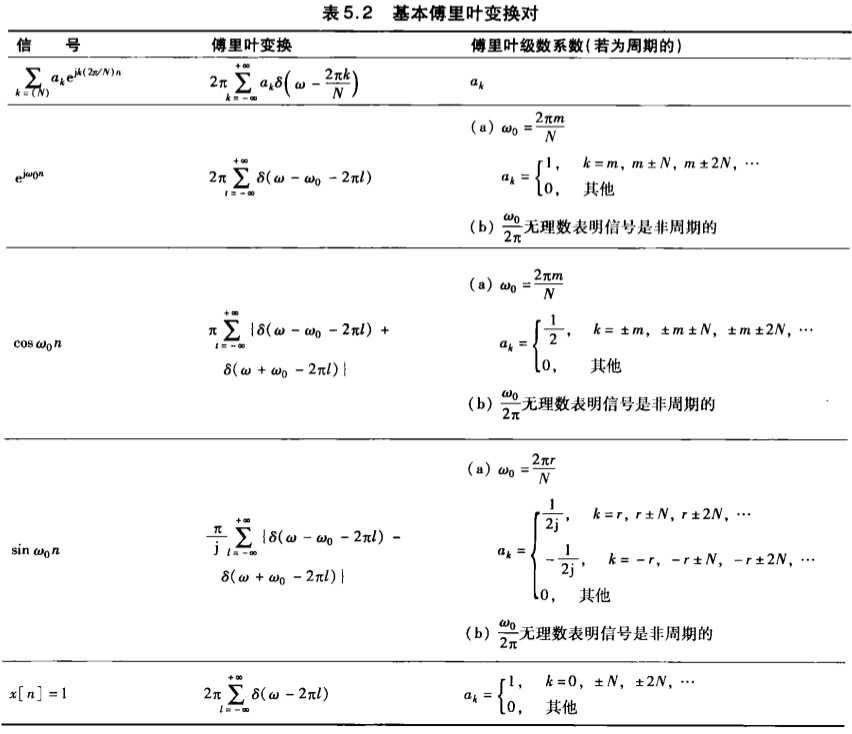
\includegraphics[scale=.32]{ss-c-t5-2a}
    \end{center}
  \end{frame}  
   
  %% PAGE
  \begin{frame}
    \frametitle{基本傅立叶变换对}
    \begin{center}
      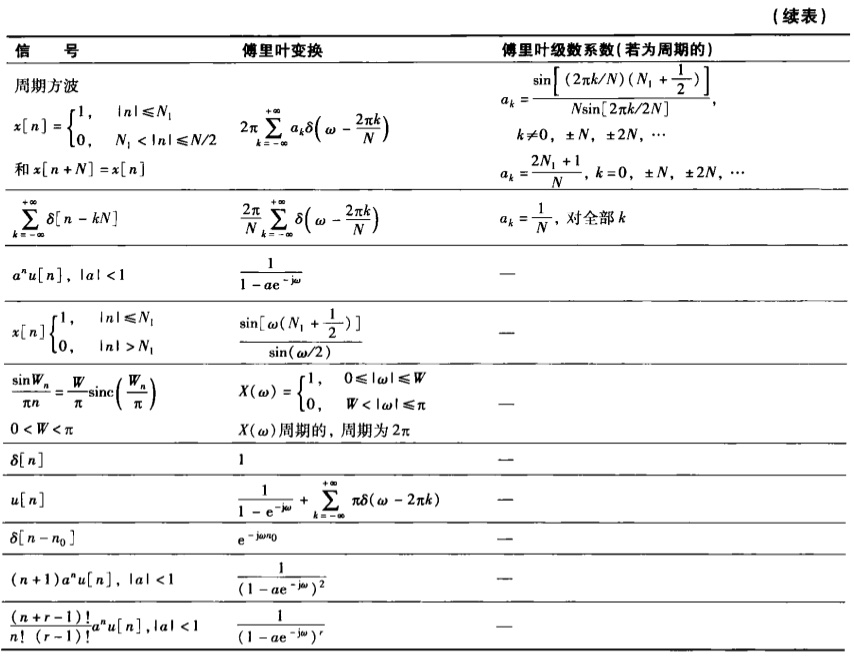
\includegraphics[scale=.32]{ss-c-t5-2b}
    \end{center}
  \end{frame}      
    
  %% PAGE
  \begin{frame}
    \frametitle{Questions}
    \begin{itemize}
    \item Any questions?
    \end{itemize}
    \begin{center}
      
\includegraphics[scale=.5]{question}
    \end{center}
  \end{frame}       
        
	\section{离散时间傅立叶变换的性质}

  %% PAGE
  \begin{frame}
    \frametitle{性质}
    \begin{itemize}
    \item 周期
    \[
    	X(e^{j(\omega+2\pi)})=X(e^{j\omega})
	\]
    \item 时移
    \[
    	x[n-n_0] \xleftrightarrow{\mathscr{F}} e^{-j\omega n_0}X(e^{j\omega})
	\]
    \item 频移
    \[
    	e^{j\omega_0 n}x[n] \xleftrightarrow{\mathscr{F}} X(e^{j(\omega-\omega_0)})
	\]	
	例子
    	\begin{itemize}
    	\item 理想高通滤波器是理想低通滤波器的半个周期(即$\pi$)频移 \\
	\begin{tabular}{ll}
	\raisebox{-.5\height}

$H_{hp}(e^{j\omega})=H_{lp}(e^{j(\omega-\pi)})$

&
    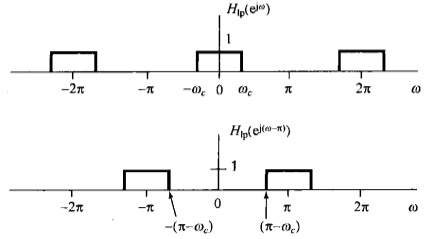
\includegraphics[valign=m,scale=.28]{ss-c-f5-12}    \\
    \end{tabular}  
    	
		\item 因为LTI系统的频率响应$H(e^{j\omega})$是单位脉冲响应$h[n]$的傅立叶变换
		\[
			H(e^{j\omega})=\mathscr{F}(h[n])=\sum_n h[n]e^{-j\omega n}
		\]
		所以$h_{hp}[n]=e^{j\pi n}h_{lp}[n]=(-1)^nh_{lp}[n]$
		
    	\end{itemize}
	
	\end{itemize}
  \end{frame}   
  	 
  %% PAGE
  \begin{frame}
    \frametitle{性质}
    \begin{itemize}
    \item 卷积
    \[
    	x_1[n] \ast x_2[n] \xleftrightarrow{\mathscr{F}} X_1(e^{j\omega})X_2(e^{j\omega})
	\]    
    \item 相乘
    \[
    	x_1[n]x_2[n] \xleftrightarrow{\mathscr{F}} \frac{1}{2\pi}\int_{2\pi}X_1(e^{j\theta})X_2(e^{j(\omega-\theta)})d\theta = X_1(e^{j\omega}) \circledast X_2(e^{j\omega})
	\] 	
		\begin{itemize}
		\item 注意:右边是周期卷积
		\end{itemize}
	\end{itemize}
  \end{frame}   
	
  %% PAGE
  \begin{frame}
    \frametitle{性质}
    \begin{itemize}
    \item 对偶
    \end{itemize}
    \begin{center}
      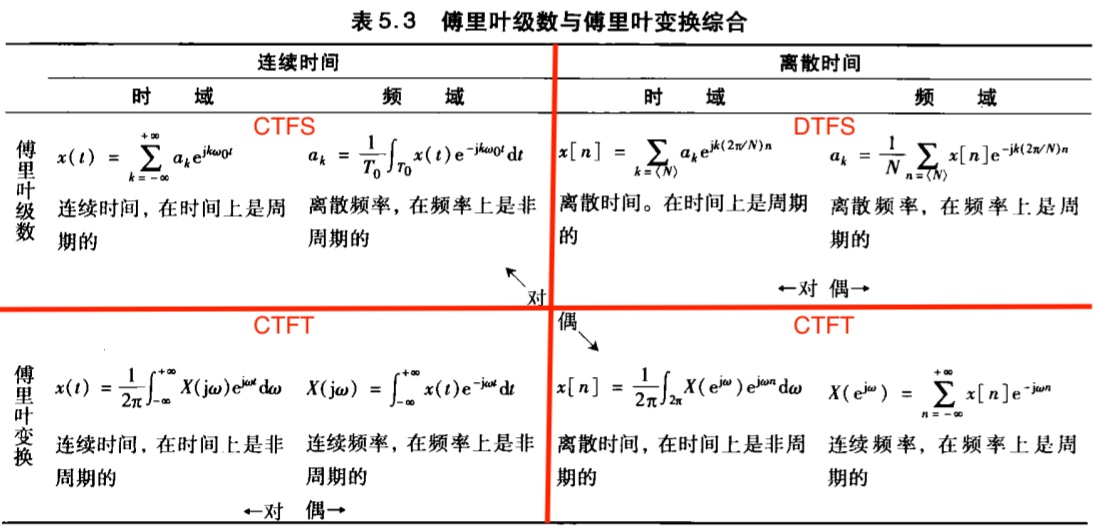
\includegraphics[scale=.32]{ss-c-t5-3}
    \end{center}
  \end{frame}  
  	        
  %% PAGE
  \begin{frame}
    \frametitle{Questions}
    \begin{itemize}
    \item Any questions?
    \end{itemize}
    \begin{center}
      
\includegraphics[scale=.5]{question}
    \end{center}
  \end{frame} 
  	        
\ifxetexorluatex\else
\end{CJK*}
\fi
\end{document}

%%% Local Variables: 
%%% mode: latex
%%% TeX-master: t
%%% End: 
